MPEG-7 es un estándar para la descripción de contenido multimedia, que define un conjunto de atributos simples y de bajo nivel con el propósito de caracterizar cualquier tipo de sonido.
Este conjunto está constituido por 17 características asociadas a toda señal de sonido~\cite{Kim05,Manjunath02}.
A continuación presentamos una descripción de estas, agrupándolas de acuerdo al modo en que describen la señal.

\subsection{Descriptores básicos}\label{subsec:descriptoresBásicos}

Las dos características de esta categoría describen las propiedades de la señal en el dominio del tiempo de forma simple;
el costo computacional de calcularlas es bajo.

\subsubsection{Audio Waveform}

Para computar esta característica se divide la señal en tramas no superpuestas ($M = N$), y se computan, por cada trama, los 2 valores siguientes:

\begin{itemize}
    \item Menor valor de amplitud de la señal presente en la trama.
    \item Mayor valor de amplitud de la señal presente en la trama.
\end{itemize}

El \textit{audio waveform} (AWF) de la señal consistirá en un vector con los pares calculados, correspondientes a cada una de dichas tramas.

La extracción de esta característica puede ser vista como un modo de <<compresión>> de la señal.
Si se toma $N=1$ se obtendrá la propia señal, mientras que a medida que se seleccionen valores de $N$ más altos, el número de valores resultantes será cada vez menor, obteniéndose una representación reducida de la señal original.
El AWF puede representarse gráficamente como un conjunto de segmentos con extremos en los valores de la tupla correspondiente y desplazados en el tiempo relativo a su posición en la señal (figura~\ref{img:awf+ap}).

\subsubsection{Audio Power}

El \textit{audio power} (AP) describe el comportamiento de la potencia de la señal en cada instante de tiempo.
Al igual que para la AWF, su cálculo requiere dividir la señal en tramas no superpuestas;
y se computa, para la trama $x[n]$ mediante la siguiente expresión:

\begin{equation}
    \label{eq:AP}
    AP = \frac{1}{N}\sum_{n=0}^{N-1}{|x[n]|^2}
\end{equation}

La representación gráfica del AP posibilita el análisis directo de la evolución de la amplitud de la señal en el transcurso del tiempo, lo que puede observarse en la figura~\ref{img:awf+ap}.

\begin{figure}[!h]
    \centering
    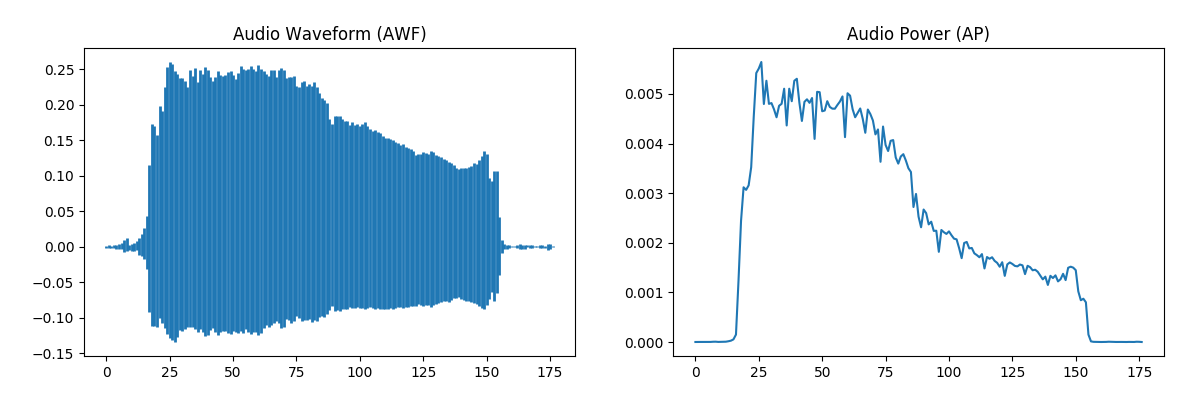
\includegraphics[width=\textwidth]{awf+ap.png}
    \caption{Características básicas de una señal de audio según MPEG-7 (tramas de 1024 muestras).}
    \label{img:awf+ap}
\end{figure}

\subsection{Descriptores espectrales básicos}\label{subsec:descriptoresEspectralesBásicos}

Las características de esta categoría describen la representación de las señales de sonido en el dominio de las frecuencias.
Requieren la división de la señal en tramas, en algunos casos producen un vector de características por cada trama, y en otros un único valor;
el resultado correspondiente a la señal completa será entonces una matriz para los primeros, o un vector para los segundos.

Una trama $x[n]$, de longitud $N$, tiene una representación en el dominio de las frecuencias que puede ser obtenida mediante la aplicación de la transformada discreta de Fourier (DFT por sus siglas en inglés):

\begin{equation}
    \label{eq:DFT}
    X[f] = \sum_{n=0}^{N-1}{x[n]e^{\frac{-i2\pi fn}{N}}}
\end{equation}

El espectro $X[f]$ puede ser transformado de vuelta al dominio del tiempo aplicando la transformada discreta inversa de Fourier (IDFT):

\begin{equation}
    \label{eq:IDFT}
    x[n] = \frac{1}{N}\sum_{f=0}^{N-1}{X[f]e^{\frac{i2\pi fn}{N}}}
\end{equation}

Al ser $x[n]$ un vector de valores reales, podemos aplicar sobre este una propiedad de la DFT que plantea que el vector $X[f]$ es, por tanto, conjugado simétrico, por lo que suelen considerarse solamente los últimos $\lceil (N+1)/2 \rceil$ valores de este.

La posición $k$-ésima del vector $X[k]$ contiene la amplitud correspondiente a la frecuencia $k(F_s/N)$ en la señal.

Podemos definir $X[f,t]$ como la matriz compuesta por las DFTs correspondientes a cada una de las tramas de una señal, donde el valor en la posición $(f, t)$ corresponde a la amplitud de la frecuencia $f$ en la trama $t$.
A partir de esta matriz se construye el espectrograma de la señal.

\subsubsection{Audio Spectrum Envelope}

El \textit{audio spectrum envelope} (ASE) constituye una reducción del espectrograma de acuerdo a la percepción del sonido en los seres humanos.
Para ello, se agrupan las frecuencias del espectro en \textbf{bandas}, distribuidas logarítmicamente entre dos valores extremos $loEdge$ (inferior) y $hiEdge$ (superior);
de esta forma, se convertirá la señal del espectro de frecuencias al de \textit{log-frecuencias}.

Para la determinación de las bandas se define un valor $r$ conocido como \textbf{resolución espectral}, que puede tomar ocho posibles valores, dados por la expresión:

\[
    r = 2^j (-4\leq j \leq 3)
\]

Asimismo, los valores $loEdge$ y $hiEdge$ deberán ser múltiplos o divisores de 1 kHz dados por la expresión $2^p \cdot 1$ kHz, $p \in \mathbb{Z}$.
Generalmente 62.5 Hz y 16 kHz son los valores seleccionados para $loEdge$ y $hiEdge$ respectivamente.

Los valores extremos $loF_b$ y $hiF_b$ de la banda $b$ se calculan mediante las expresiones:

\begin{gather*}
    loF_b = loEdge \cdot 2^{(b-1)r} \\
    hiF_b = loEdge \cdot 2^{br}
\end{gather*}

Luego, se establece un mapeo entre la DFT de la señal y su ASE, donde la amplitud de cada frecuencia presente en la DFT es sumada al coeficiente de la banda correspondiente en el ASE\@.
El estándar MPEG-7 no especifica el procedimiento en caso de que alguna frecuencia se encuentre en el límite entre dos bandas;
el enfoque más simple consiste en distribuir su amplitud equitativamente entre estas.

Adicionalmente, se incluyen 2 coeficientes correspondientes a los intervalos $[0, loEdge)$ y $(hiEdge, F_s/2]$, añadidos al inicio y final del vector de características respectivamente.

\subsubsection{Audio Spectrum Centroid}

El \textit{audio spectrum centroid} (ASC) constituye el centro de gravedad del espectro de frecuencias de una trama, y permite describir la señal en términos del tipo de frecuencias predominantes (altas o bajas) en cada trama.
Existen variantes para su cálculo, siendo muy populares la que se hace a partir de la DFT de la trama, y la que emplea su ASE;
mostradas en las ecuaciones (\ref{eq:ASC-DFT}) y (\ref{eq:ASC-ASE}) respectivamente:

\begin{equation}
    \label{eq:ASC-DFT}
    ASC = \frac{\sum_{k=0}^{K_{DFT}-1}{f(k)|X[k]|}}{\sum_{k=0}^{K-1}{|X[k]|}}
\end{equation}

\noindent
donde $K_{DFT}$ es la longitud del vector correspondiente a la DFT de la trama, y $f(k)$ frecuencia asociada a la posición $k$-ésima de este.

\begin{equation}
    \label{eq:ASC-ASE}
    ASC = \frac{\sum_{k=0}^{K_{ASE}-1}{k\cdot ASE_k}}{\sum_{k=0}^{K-1}{ASE_k}}
\end{equation}

\noindent
donde $K_{ASE}$ es la longitud del vector correspondiente al ASE de la trama.
El valor obtenido aplicando esta ecuación estará dado en términos de la posición de la frecuencia centroide dentro de las bandas de log-frecuencias.
Si se desea llevar al espectro de frecuencias, se multiplica su diferencia con el extremo inferior de la banda correspondiente por la diferencia entre ambos extremos de esta, y luego se suma el valor obtenido al extremo inferior, siendo el resultado de esta operación la expresión del centroide en hertz.

El estándar MPEG-7 define el ASC mediante la variante presentada en la ecuación~(\ref{eq:ASC-ASE}).

\subsubsection{Audio Spectrum Spread}

También conocido como \textit{instantaneous bandwith} o \textit{spectral width}, el \textit{audio spectrum spread} (ASS) de una señal refleja la dispersión del espectro de log-frecuencias en torno a su centroide.
En MPEG-7 se le define como el segundo momento central del ASE\@.

Puede calcularse aplicando la siguiente expresión en cada trama:

\begin{equation}
    \label{eq:ASS}
    ASS = \sqrt{\frac{\sum_{k=0}^{K-1}{\left[ \log_{2}{(f(k))-ASC} \right]^2 ASE_k}}{\sum_{k=0}^{K-1}{ASE_k}}}
\end{equation}

\noindent
donde $K$ es el tamaño del vector correspondiente al ASE de la trama.

Valores bajos (característicos de sonidos harmónicos) del ASS expresan una concentración de las amplitudes alrededor de la frecuencia centroide;
los valores altos (propios de ruidos), en cambio, muestran una dispersión de las amplitudes en un rango de frecuencias mayor.

\subsubsection{Audio Spectrum Flatness}

El \textit{audio spectrum flatness} (ASF) de una señal refleja su similitud a una señal compuesta por ruido, caso en que su valor se aproxima a 1;
mientras que si se trata de una señal harmónica, el valor será próximo a 0.

Para calcular el ASF, de acuerdo con el estándar MPEG-7, se divide la señal en tramas no superpuestas, y el espectro se separa en bandas con $loEdge = 250$ Hz y $hiEdge = 16$ kHz.
Los extremos de cada banda se determinan por las ecuaciones:

\begin{gather*}
    loF_b = 0.95 \cdot loEdge \cdot 2^{\frac{1}{4}(b-1)} \\
    hiF_b = 1.05 \cdot loEdge \cdot 2^{\frac{1}{4}b}
\end{gather*}

Los coeficientes $0.95$ y $1.05$ por los que se multiplica $loEdge$ tienen como finalidad producir una superposición entre bandas adyacentes.

El coeficiente correspondiente a la banda $b$ en el ASF se calcula como la razón entre las medias geométrica y aritmética de las amplitudes presentes en esta, es decir, mediante la expresión:

\begin{equation}
    \label{eq:ASF}
    ASF_b = \frac{\prod_{k=0}^{K-1}{|X_{b}[k]|}}{\frac{1}{K}\sum{k=0}^{K-1}{|X_{b}[k]|}}
\end{equation}

\noindent
donde $X_{b}[k]$ es la subsecuencia de la DFT de la señal correspondiente a las frecuencias que pertenecen a la banda $b$, y $K$ su cardinalidad.

La matriz de los ASF es un buen identificador para una señal, y el vector formado por los promedios de los ASF de cada trama puede ser empleado como vector de características en aplicaciones de clasificación de señales de audio~\cite{Kim05}.

\begin{figure}[!h]
    \centering
    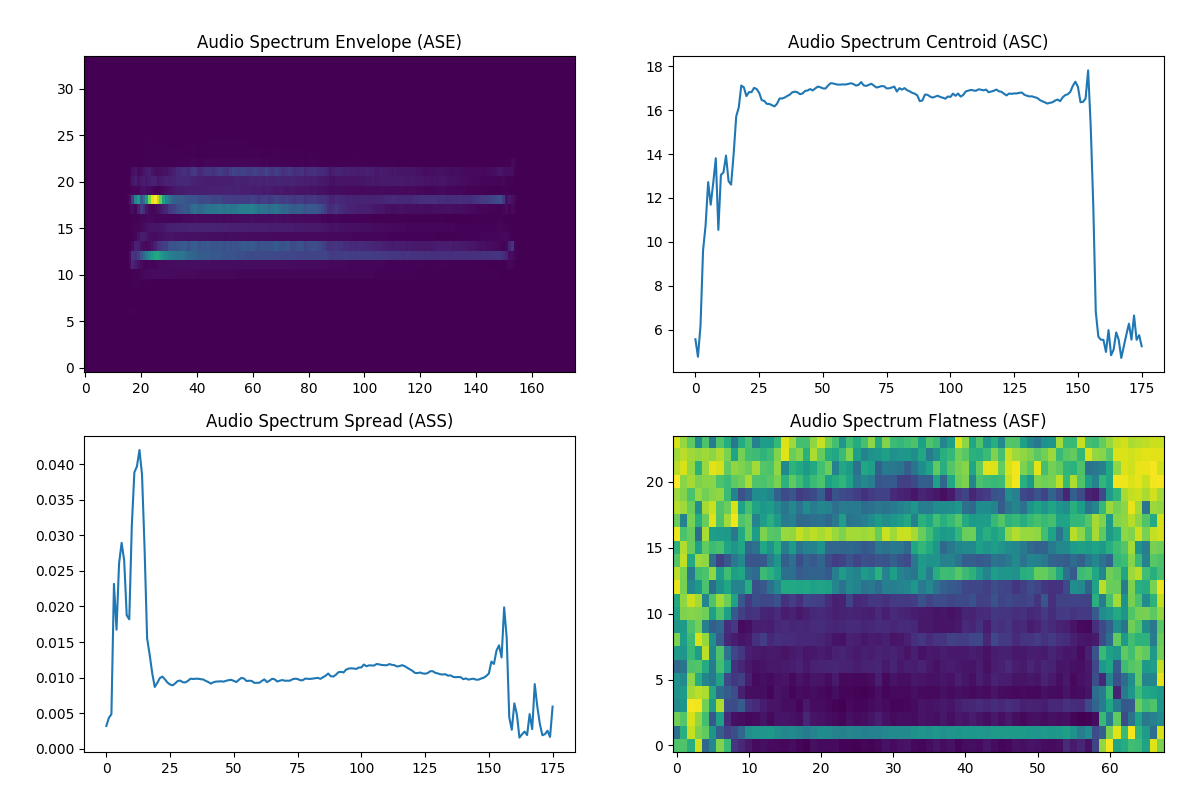
\includegraphics[width=0.9\textwidth]{basic-spectral-descriptors.png}
    \caption{Características espectrales básicas de una señal de audio según MPEG-7.}
    \label{img:basic-spectral-descriptors}
\end{figure}